\documentclass[12pt, a4paper]{article}

\usepackage[margin=1.1in]{geometry}

\usepackage[utf8]{inputenc}
\usepackage[square,numbers]{natbib}
\usepackage{hyperref}

\usepackage{amsfonts}
\usepackage{graphicx}
\usepackage{subfig}

\pagenumbering{gobble}

\begin{document}

\large
\noindent \textbf{Hathor Network\footnote{\url{https://hathor.network/} | \href{contact@hathor.network}{contact@hathor.network} | Written on \today}}

\normalsize
\noindent \emph{A Novel, Scalable, and Decentralized Architecture for a General Distributed Ledger}

\vspace{1em}

Hathor is a transactional consensus platform comprised of an entirely novel architecture, based on concepts from both direct acyclic graph (DAG) and blockchain technologies combined. \textbf{We solve the problems of scalability and decentralization maintenance among distributed ledger networks} by including a chain of mined blocks inside a DAG of transactions. The blockchain ensures security when the number of transactions per second is small, whereas the DAG prevails when the number increases significantly.

A highly scalable distributed ledger where transactions can be processed for multiple purposes with no fees will be created through its own network. At the same time, mining rewards in the form of newly generated tokens will enforce a fair distribution of economic and computational resources through decentralization and 99.99\% uptime without any form of central coordination. \textbf{Hathor is the direct result of 7+ years of academic research from its founding members,} throughout which they have been stress-testing its assumptions and alpha versions.

We see scalability as a significant challenge in cryptocurrencies. IOTA made great strides towards scalability, but their solution does not seem to work when the number of transactions per second is small. Hathor’s architecture lies between the ones from Bitcoin and IOTA and presents a solution to scaling, centralization and spam issues.

By the academic research conducted by Dr. Marcelo Brogliato and published as part of his Ph.D. thesis, we have a detailed analysis of Hathor's architecture through simulations. \textbf{The primary result is that it works correctly under any number of transactions per second.} The higher the number of transactions per second, the faster new transactions are confirmed.

As in IOTA, new transactions confirm previous ones, forming a DAG. Each transaction has its own proof-of-work which is solved by the issuer before propagating the transactions in the network. As in the case of Bitcoin, miners find new blocks which form a blockchain inside the DAG. Blocks collect newly generated tokens and confirm all the transactions in the DAG. Each transaction has an accumulated weight which expresses the necessary effort to break the transaction, similar to the number of confirmations in Bitcoin.

\vspace{1em}
\noindent \textbf{Hathor Foundation}

In the coming months, we will start the Hathor Foundation as a way to raise funds to be used for research, partnerships, regulation, education, and development related to Hathor and its emerging ecosystem. Although there are a few details yet to be discussed, we plan to do a pre-sale of Hathor's genesis tokens, which would be created when the network is launched. \textbf{Our first round goal is to raise \$5MM to open the foundation,} sign vesting contracts with developers and advisors and launch the network. Investors would also have votes in the foundation's board.

\clearpage

\begin{figure}[!htb]
\centering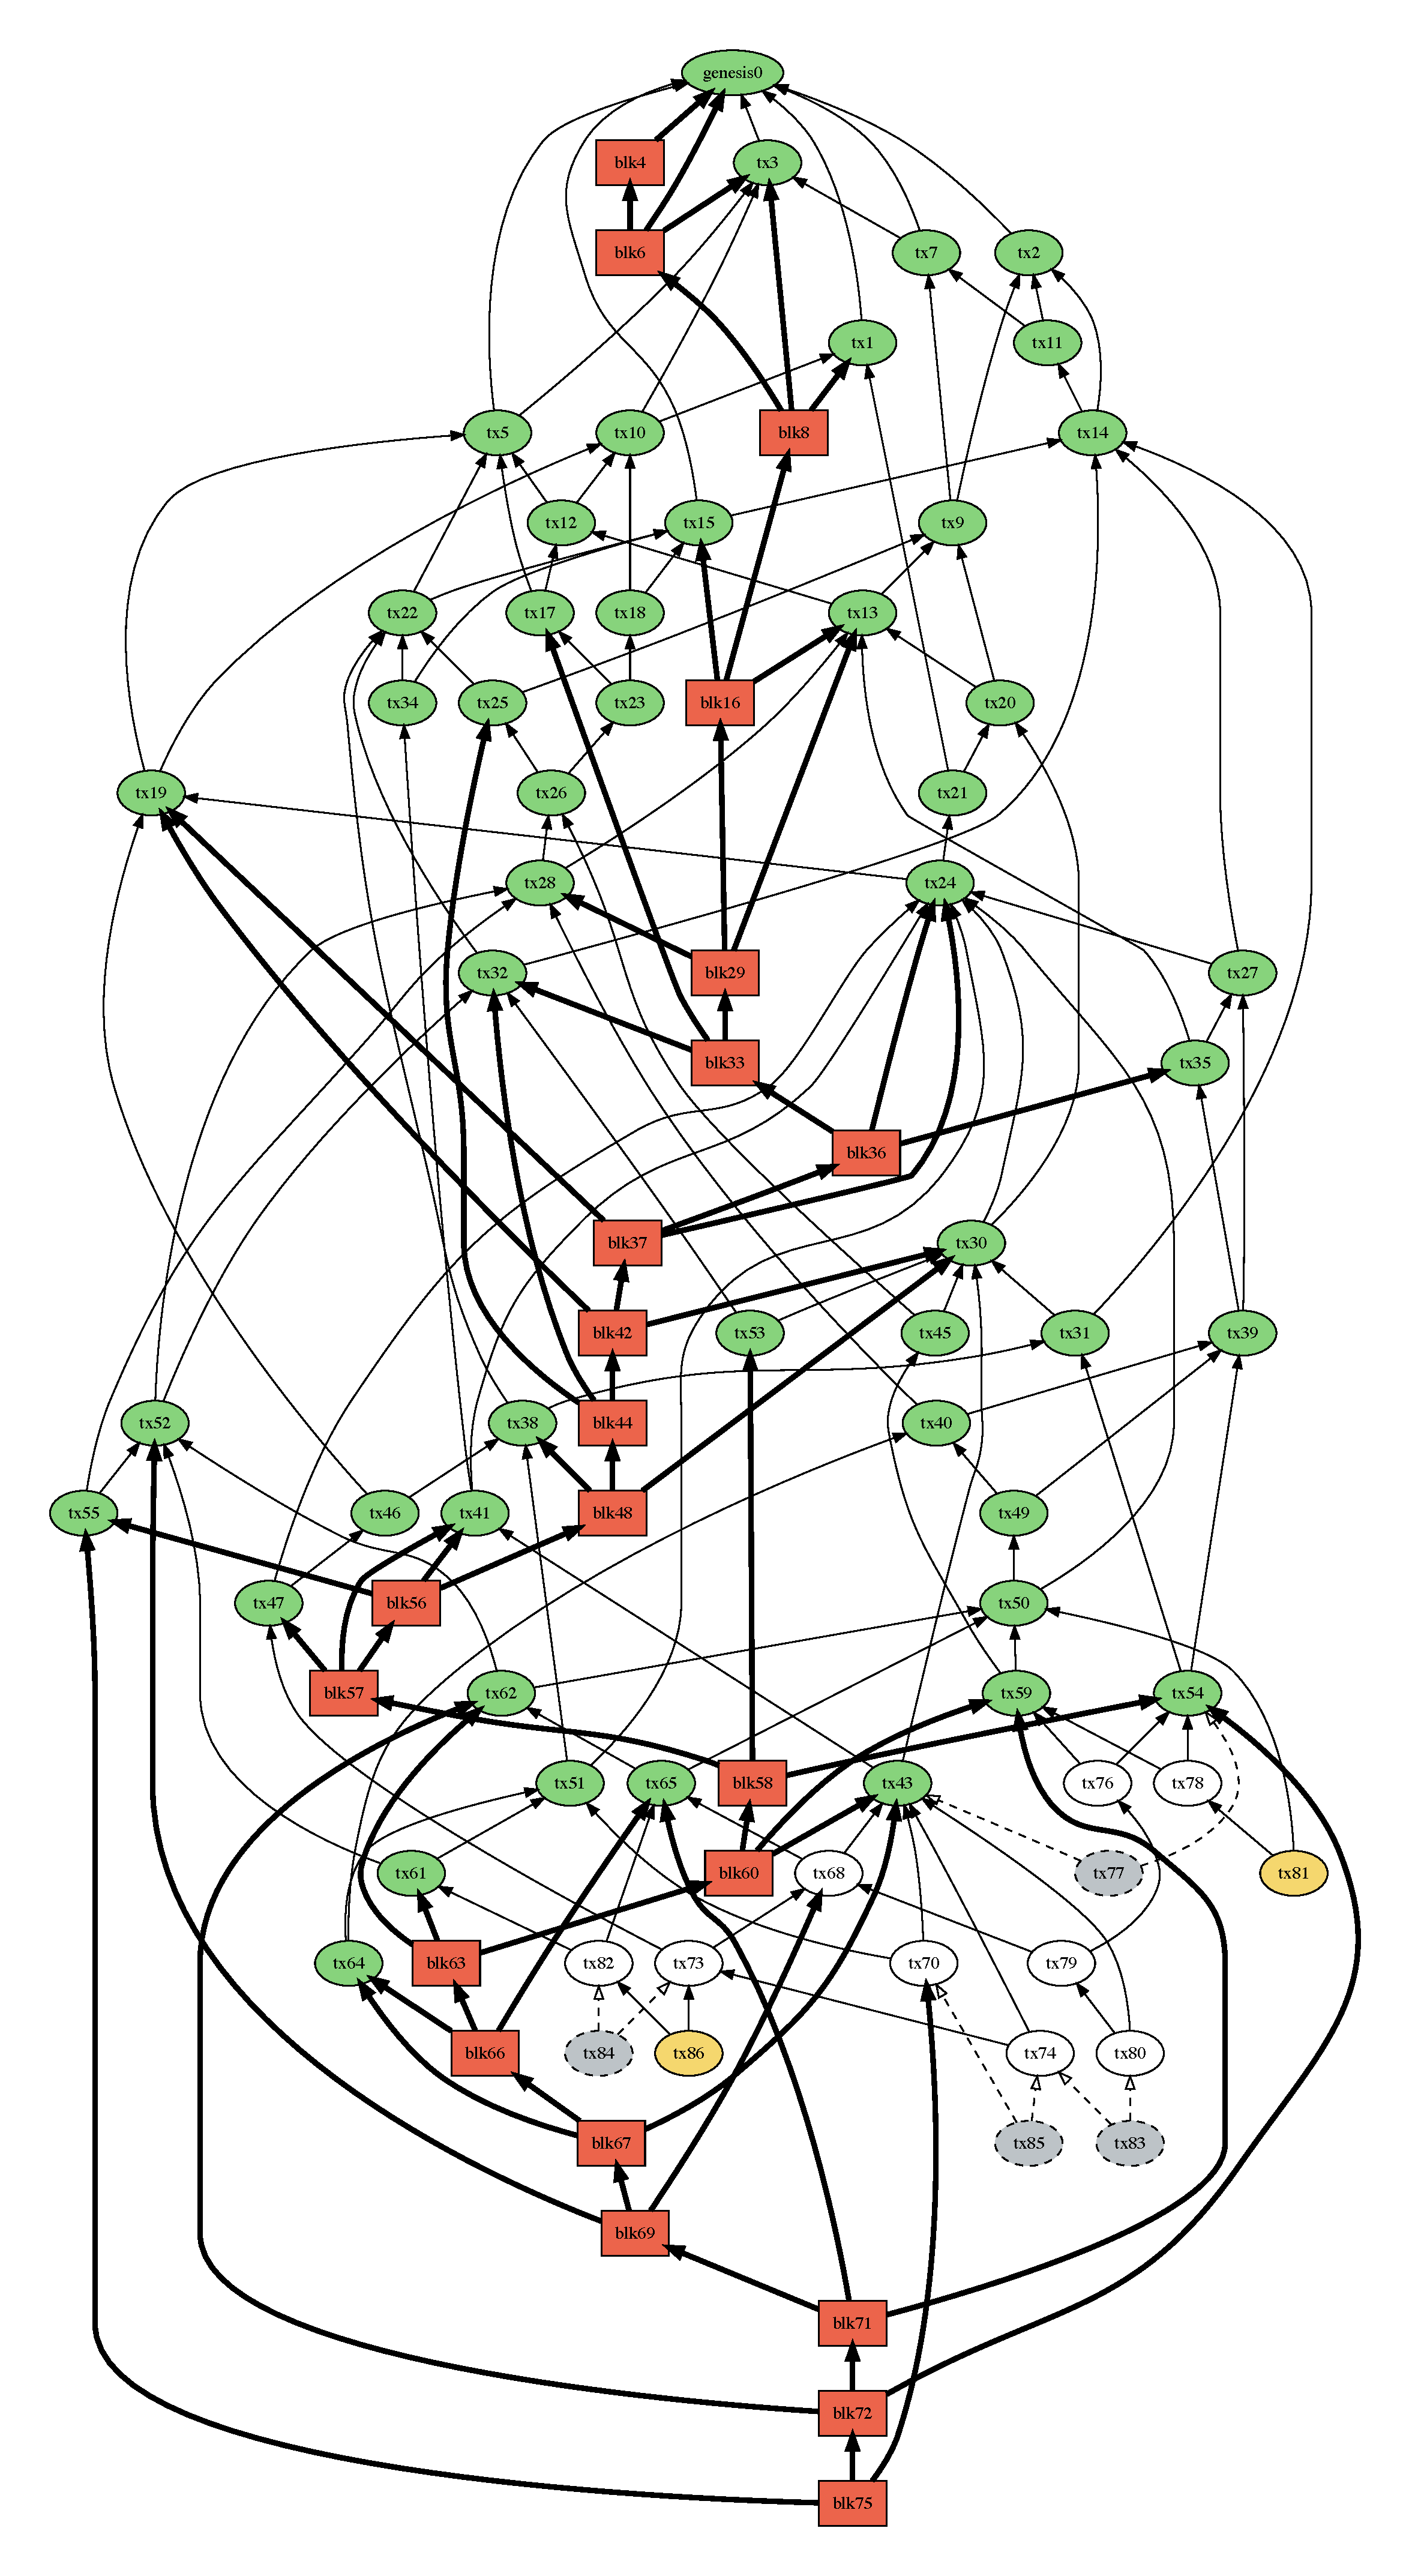
\includegraphics[width=0.8\textwidth]{./images01/sim/hathor-2.pdf}
\caption{Visualization of a Hathor's graph with transactions and blocks. Red boxes are blocks; green circles are confirmed transactions; white circles are in-progress transactions; yellow circles are unconfirmed transactions (tips); and grey circles are transactions solving the proof-of-work which have not been propagated yet. The arrows show the confirmation chain. Block's arrows are in bold. \label{fig:hathor-dag-big}}
\end{figure}

\end{document}
